% !Mode:: "TeX:UTF-8"
\documentclass[12pt,a4paper]{article}

%%%%%%%%------------------------------------------------------------------------
%%%% 日常所用宏包

%% 控制页边距
% 如果是beamer文档类, 则不用geometry
\makeatletter
\@ifclassloaded{beamer}{}{\usepackage[top=2.5cm, bottom=2.5cm, left=2.5cm, right=2.5cm]{geometry}}
\makeatother

%% 控制项目列表
\usepackage{enumerate}

%% 多栏显示
\usepackage{multicol}

%% 算法环境
\usepackage{algorithm}  
\usepackage{algorithmic} 
\usepackage{float} 

%% 网址引用
\usepackage{url}

%% 控制矩阵行距
\renewcommand\arraystretch{1.4}

%% hyperref宏包,生成可定位点击的超链接,并且会生成pdf书签
\makeatletter
\@ifclassloaded{beamer}{
\usepackage{hyperref}
\usepackage{ragged2e} % 对齐
}{
\usepackage[%
    pdfstartview=FitH,%
    CJKbookmarks=true,%
    bookmarks=true,%
    bookmarksnumbered=true,%
    bookmarksopen=true,%
    colorlinks=true,%
    citecolor=blue,%
    linkcolor=blue,%
    anchorcolor=green,%
    urlcolor=blue%
]{hyperref}
}
\makeatother



\makeatletter % 如果是 beamer 不需要下面两个包
\@ifclassloaded{beamer}{
\mode<presentation>
{
} 
}{
%% 控制标题
\usepackage{titlesec}
%% 控制目录
\usepackage{titletoc}
}
\makeatother

%% 控制表格样式
\usepackage{booktabs}

%% 控制字体大小
\usepackage{type1cm}

%% 首行缩进,用\noindent取消某段缩进
\usepackage{indentfirst}

%% 支持彩色文本、底色、文本框等
\usepackage{color,xcolor}

%% AMS LaTeX宏包: http://zzg34b.w3.c361.com/package/maths.htm#amssymb
\usepackage{amsmath,amssymb}
%% 多个图形并排
\usepackage{subfig}
%%%% 基本插图方法
%% 图形宏包
\usepackage{graphicx}
\newcommand{\red}[1]{\textcolor{red}{#1}}
\newcommand{\blue}[1]{\structure{#1}}
\newcommand{\brown}[1]{\textcolor{brown}{#1}}
\newcommand{\green}[1]{\textcolor{green}{#1}}


%%%% 基本插图方法结束

%%%% pgf/tikz绘图宏包设置
\usepackage{pgf,tikz}
\usetikzlibrary{shapes,automata,snakes,backgrounds,arrows}
\usetikzlibrary{mindmap}
%% 可以直接在latex文档中使用graphviz/dot语言,
%% 也可以用dot2tex工具将dot文件转换成tex文件再include进来
%% \usepackage[shell,pgf,outputdir={docgraphs/}]{dot2texi}
%%%% pgf/tikz设置结束


\makeatletter % 如果是 beamer 不需要下面两个包
\@ifclassloaded{beamer}{

}{
%%%% fancyhdr设置页眉页脚
%% 页眉页脚宏包
\usepackage{fancyhdr}
%% 页眉页脚风格
\pagestyle{plain}
}

%% 有时会出现\headheight too small的warning
\setlength{\headheight}{15pt}

%% 清空当前页眉页脚的默认设置
%\fancyhf{}
%%%% fancyhdr设置结束


\makeatletter % 对 beamer 要重新设置
\@ifclassloaded{beamer}{

}{
%%%% 设置listings宏包用来粘贴源代码
%% 方便粘贴源代码,部分代码高亮功能
\usepackage{listings}

%% 设置listings宏包的一些全局样式
%% 参考http://hi.baidu.com/shawpinlee/blog/item/9ec431cbae28e41cbe09e6e4.html
\lstset{
showstringspaces=false,              %% 设定是否显示代码之间的空格符号
numbers=left,                        %% 在左边显示行号
numberstyle=\tiny,                   %% 设定行号字体的大小
basicstyle=\footnotesize,                    %% 设定字体大小\tiny, \small, \Large等等
keywordstyle=\color{blue!70}, commentstyle=\color{red!50!green!50!blue!50},
                                     %% 关键字高亮
frame=shadowbox,                     %% 给代码加框
rulesepcolor=\color{red!20!green!20!blue!20},
escapechar=`,                        %% 中文逃逸字符,用于中英混排
xleftmargin=2em,xrightmargin=2em, aboveskip=1em,
breaklines,                          %% 这条命令可以让LaTeX自动将长的代码行换行排版
extendedchars=false                  %% 这一条命令可以解决代码跨页时,章节标题,页眉等汉字不显示的问题
}}
\makeatother
%%%% listings宏包设置结束


%%%% 附录设置
\makeatletter % 对 beamer 要重新设置
\@ifclassloaded{beamer}{

}{
\usepackage[title,titletoc,header]{appendix}
}
\makeatother
%%%% 附录设置结束


%%%% 日常宏包设置结束
%%%%%%%%------------------------------------------------------------------------


%%%%%%%%------------------------------------------------------------------------
%%%% 英文字体设置结束
%% 这里可以加入自己的英文字体设置
%%%%%%%%------------------------------------------------------------------------

%%%%%%%%------------------------------------------------------------------------
%%%% 设置常用字体字号,与MS Word相对应

%% 一号, 1.4倍行距
\newcommand{\yihao}{\fontsize{26pt}{36pt}\selectfont}
%% 二号, 1.25倍行距
\newcommand{\erhao}{\fontsize{22pt}{28pt}\selectfont}
%% 小二, 单倍行距
\newcommand{\xiaoer}{\fontsize{18pt}{18pt}\selectfont}
%% 三号, 1.5倍行距
\newcommand{\sanhao}{\fontsize{16pt}{24pt}\selectfont}
%% 小三, 1.5倍行距
\newcommand{\xiaosan}{\fontsize{15pt}{22pt}\selectfont}
%% 四号, 1.5倍行距
\newcommand{\sihao}{\fontsize{14pt}{21pt}\selectfont}
%% 半四, 1.5倍行距
\newcommand{\bansi}{\fontsize{13pt}{19.5pt}\selectfont}
%% 小四, 1.5倍行距
\newcommand{\xiaosi}{\fontsize{12pt}{18pt}\selectfont}
%% 大五, 单倍行距
\newcommand{\dawu}{\fontsize{11pt}{11pt}\selectfont}
%% 五号, 单倍行距
\newcommand{\wuhao}{\fontsize{10.5pt}{10.5pt}\selectfont}
%%%%%%%%------------------------------------------------------------------------


%% 设定段间距
\setlength{\parskip}{0.5\baselineskip}

%% 设定行距
\linespread{1}


%% 设定正文字体大小
% \renewcommand{\normalsize}{\sihao}

%制作水印
\RequirePackage{draftcopy}
\draftcopyName{XTUMESH}{100}
\draftcopySetGrey{0.90}
\draftcopyPageTransform{40 rotate}
\draftcopyPageX{350}
\draftcopyPageY{80}

%%%% 个性设置结束
%%%%%%%%------------------------------------------------------------------------


%%%%%%%%------------------------------------------------------------------------
%%%% bibtex设置

%% 设定参考文献显示风格
% 下面是几种常见的样式
% * plain: 按字母的顺序排列,比较次序为作者、年度和标题
% * unsrt: 样式同plain,只是按照引用的先后排序
% * alpha: 用作者名首字母+年份后两位作标号,以字母顺序排序
% * abbrv: 类似plain,将月份全拼改为缩写,更显紧凑
% * apalike: 美国心理学学会期刊样式, 引用样式 [Tailper and Zang, 2006]

\makeatletter
\@ifclassloaded{beamer}{
\bibliographystyle{apalike}
}{
\bibliographystyle{unsrt}
}
\makeatother


%%%% bibtex设置结束
%%%%%%%%------------------------------------------------------------------------

%%%%%%%%------------------------------------------------------------------------
%%%% xeCJK相关宏包

\usepackage{xltxtra,fontspec,xunicode}
\usepackage[slantfont, boldfont]{xeCJK} 
\usepackage{bm}

\setlength{\parindent}{2em}%中文缩进两个汉字位

%% 针对中文进行断行
\XeTeXlinebreaklocale "zh"             

%% 给予TeX断行一定自由度
\XeTeXlinebreakskip = 0pt plus 1pt minus 0.1pt

%%%% xeCJK设置结束                                       
%%%%%%%%------------------------------------------------------------------------

%%%%%%%%------------------------------------------------------------------------
%%%% xeCJK字体设置

%% 设置中文标点样式,支持quanjiao、banjiao、kaiming等多种方式
\punctstyle{kaiming}                                        
                                                     
%% 设置缺省中文字体
%\setCJKmainfont[BoldFont={Adobe Heiti Std}, ItalicFont={Adobe Kaiti Std}]{Adobe Song Std}   
\setCJKmainfont{SimSun}
%% 设置中文无衬线字体
%\setCJKsansfont[BoldFont={Adobe Heiti Std}]{Adobe Kaiti Std}  
%% 设置等宽字体
%\setCJKmonofont{Adobe Heiti Std}                            

%% 英文衬线字体
\setmainfont{DejaVu Serif}                                  
%% 英文等宽字体
\setmonofont{DejaVu Sans Mono}                              
%% 英文无衬线字体
\setsansfont{DejaVu Sans}                                   

%% 定义新字体
\setCJKfamilyfont{song}{Adobe Song Std}                     
\setCJKfamilyfont{kai}{Adobe Kaiti Std}
\setCJKfamilyfont{hei}{Adobe Heiti Std}
\setCJKfamilyfont{fangsong}{Adobe Fangsong Std}
\setCJKfamilyfont{lisu}{LiSu}
\setCJKfamilyfont{youyuan}{YouYuan}

%% 自定义宋体
\newcommand{\song}{\CJKfamily{song}}                       
%% 自定义楷体
\newcommand{\kai}{\CJKfamily{kai}}                         
%% 自定义黑体
\newcommand{\hei}{\CJKfamily{hei}}                         
%% 自定义仿宋体
\newcommand{\fangsong}{\CJKfamily{fangsong}}               
%% 自定义隶书
\newcommand{\lisu}{\CJKfamily{lisu}}                       
%% 自定义幼圆
\newcommand{\youyuan}{\CJKfamily{youyuan}}                 

%%%% xeCJK字体设置结束
%%%%%%%%------------------------------------------------------------------------

%%%%%%%%------------------------------------------------------------------------
%%%% 一些关于中文文档的重定义
\newcommand{\chntoday}{\number\year\,年\,\number\month\,月\,\number\day\,日}
%% 数学公式定理的重定义

%% 中文破折号,据说来自清华模板
\newcommand{\pozhehao}{\kern0.3ex\rule[0.8ex]{2em}{0.1ex}\kern0.3ex}

\newtheorem{example}{例}                                   
\newtheorem{theorem}{定理}[section]                         
\newtheorem{definition}{定义}
\newtheorem{axiom}{公理}
\newtheorem{property}{性质}
\newtheorem{proposition}{命题}
\newtheorem{lemma}{引理}
\newtheorem{corollary}{推论}
\newtheorem{remark}{注解}
\newtheorem{condition}{条件}
\newtheorem{conclusion}{结论}
\newtheorem{assumption}{假设}

\makeatletter %
\@ifclassloaded{beamer}{

}{
%% 章节等名称重定义
\renewcommand{\contentsname}{目录}     
\renewcommand{\indexname}{索引}
\renewcommand{\listfigurename}{插图目录}
\renewcommand{\listtablename}{表格目录}
\renewcommand{\appendixname}{附录}
\renewcommand{\appendixpagename}{附录}
\renewcommand{\appendixtocname}{附录}
%% 设置chapter、section与subsection的格式
\titleformat{\chapter}{\centering\huge}{第\thechapter{}章}{1em}{\textbf}
\titleformat{\section}{\centering\sihao}{\thesection}{1em}{\textbf}
\titleformat{\subsection}{\xiaosi}{\thesubsection}{1em}{\textbf}
\titleformat{\subsubsection}{\xiaosi}{\thesubsubsection}{1em}{\textbf}

\@ifclassloaded{book}{

}{
\renewcommand{\abstractname}{摘要}
}
}
\makeatother

\renewcommand{\figurename}{图}
\renewcommand{\tablename}{表}

\makeatletter
\@ifclassloaded{book}{
\renewcommand{\bibname}{参考文献}
}{
\renewcommand{\refname}{参考文献} 
}
\makeatother

\floatname{algorithm}{算法}
\renewcommand{\algorithmicrequire}{\textbf{输入:}}
\renewcommand{\algorithmicensure}{\textbf{输出:}}

%%%% 中文重定义结束
%%%%%%%%------------------------------------------------------------------------

%\usepackage{mathrsfs,amsmath,amssymb,bm,amsthm}
%\usepackage{mathtools}
\usepackage{hyperref}
%%%% 基本插图方法
%% 图形宏包
\usepackage{graphicx}
%% 多个图形并排
%\usepackage{subfigure}
%% 网址引用
\usepackage{url}

%% 控制项目列表
\usepackage{enumerate}

%% 多栏显示
\usepackage{multicol}

%% 控制矩阵行距
\renewcommand\arraystretch{1.4}

%\usepackage[notref,notcite]{showkeys}

\usepackage{caption}
\usepackage{overpic}
\usepackage{epsfig}
\usepackage{xcolor}
\usepackage{indentfirst}
\usepackage{fancyhdr}
\usepackage{comment}
\usepackage{makecell, rotating}
\usepackage{fullpage}
%\mathtoolsset{showonlyrefs=true,showmanualtags=true}
%\mathtoolsset{showonlyrefs=true}

\usepackage{xkeyval}
\usepackage{todonotes}
\presetkeys{todonotes}{inline}{} 
\usepackage[draft]{changes}
\usepackage{mathtools}
\mathtoolsset{showonlyrefs}
\usepackage{lipsum}% <- For dummy text
\definechangesauthor[name={Kai Jiang}, color=blue]{jk}
%\definechangesauthor[Kai]{jk}{blue}
%\definechangesauthor[John]{JD}{blue}

\numberwithin{equation}{section}
\renewcommand {\thetable} {\thesection{}.\arabic{table}}
\renewcommand {\thefigure} {\thesection{}.\arabic{figure}}


\newcommand{\bbR}{\mathbb{R}}
\newcommand{\bbZ}{\mathbb{Z}}
\newcommand{\bbQ}{\mathbb{Q}}
\newcommand{\by}{\bm{y}}
\newcommand{\bb}{\bm{b}}
\newcommand{\bx}{\bm{x}}
\newcommand{\bn}{\bm{n}}
\newcommand{\br}{\bm{r}}
\newcommand{\bh}{\bm{h}}
\newcommand{\bk}{\bm{k}}
\newcommand{\bt}{\bm{t}}
\newcommand{\bs}{\bm{s}}
\newcommand{\bu}{\bm{u}}
\newcommand{\bM}{\bm{M}}
\newcommand{\bP}{\bm{P}}
\newcommand{\bQ}{\bm{Q}}
\newcommand{\calS}{\mathcal{S}}
\newcommand{\hF}{\hat{F}}
\newcommand{\bq}{\bm{q}}
\newcommand{\hw}{\hat{w}}
\newcommand{\hphi}{\hat{\phi}}
\newcommand{\hxi}{\hat{\xi}}
\newcommand{\hJ}{\hat{J}}
\newcommand{\vzero}{\bm{0}}
%\def\bx{{\bm x}}

%%\newtheorem{proof}{Proof}[section]
%\newtheorem{thm}{Theorem}[section]
%\newtheorem{lemma}[thm]{Lemma}
%\newtheorem{proposition}[thm]{Proposition}
%\newtheorem{corollary}[thm]{Corollary}
%\newtheorem{defy}[thm]{Definition}
%\newtheorem{remark}[thm]{Remark}
%\newtheorem{sample}[thm]{Example}
%\newtheorem{assumption}[thm]{Assumption}
%\newtheorem{prop}[thm]{Properties}

\newcommand\tbbint{{-\mkern -16mu\int}}
\newcommand\tbint{{\mathchar '26\mkern -14mu\int}}
\newcommand\dbbint{{-\mkern -19mu\int}}
\newcommand\dbint{{\mathchar '26\mkern -18mu\int}}
\newcommand\bint{
{\mathchoice{\dbint}{\tbint}{\tbint}{\tbint}}
}
\newcommand\bbint{
{\mathchoice{\dbbint}{\tbbint}{\tbbint}{\tbbint}}
}


\DeclareMathOperator*{\argmin}{\mathrm{argmin}}
\DeclareMathOperator*{\argmax}{\mathrm{argmax}}

\newcommand{\Prox}{\mathrm{Prox}}
\newcommand{\GProx}{\mathrm{GProx}}

%\renewcommand{\baselinestretch}{1.5}

\numberwithin{equation}{section}
\renewcommand {\thetable} {\thesection{}.\arabic{table}}
\renewcommand {\thefigure} {\thesection{}.\arabic{figure}}
%%\newcommand{\bbR}{\mathbb{R}}
%%\newcommand{\bbZ}{\mathbb{Z}}
%%\newcommand{\bbQ}{\mathbb{Q}}
%%\newcommand{\bh}{\mathbf{h}}
%%\newcommand{\bx}{\bm{x}}
%%\newcommand{\br}{\bm{r}}
%%\newcommand{\by}{\mathbf{y}}
%%\newcommand{\bt}{\mathbf{t}}
%%\newcommand{\bs}{\mathbf{s}}
%%\newcommand{\bu}{\mathbf{u}}
%%\newcommand{\bk}{\mathbf{k}}
%%\newcommand{\bM}{\mathbf{M}}
%%\newcommand{\bP}{\mathbf{P}}
%%\newcommand{\bQ}{\mathbf{Q}}
%%\newcommand{\calS}{\mathcal{S}}
%%\newcommand{\hF}{\hat{F}}
%%\newcommand{\bq}{\mathbf{q}}
%%\newcommand{\hw}{\hat{w}}
%%\newcommand{\hphi}{\hat{\phi}}
%%\newcommand{\hxi}{\hat{\xi}}
%%\newcommand{\hJ}{\hat{J}}
%||||||| merged common ancestors
%\newcommand{\bbR}{\mathbb{R}}
%\newcommand{\bbZ}{\mathbb{Z}}
%\newcommand{\bbQ}{\mathbb{Q}}
%\newcommand{\bh}{\mathbf{h}}
%\newcommand{\bx}{\bm{x}}
\newcommand{\br}{\bm{r}}
\newcommand{\bu}{\bm{u}}
%\newcommand{\by}{\mathbf{y}}
%\newcommand{\bt}{\mathbf{t}}
%\newcommand{\bs}{\mathbf{s}}
%\newcommand{\bu}{\mathbf{u}}
\newcommand{\ba}{\mathbf{a}}
\newcommand{\bk}{\mathbf{k}}
%\newcommand{\bM}{\mathbf{M}}
%\newcommand{\bP}{\mathbf{P}}
%\newcommand{\bQ}{\mathbf{Q}}
%\newcommand{\calS}{\mathcal{S}}
%\newcommand{\hF}{\hat{F}}
%\newcommand{\bq}{\mathbf{q}}
%\newcommand{\hw}{\hat{w}}
%\newcommand{\hphi}{\hat{\phi}}
%\newcommand{\hxi}{\hat{\xi}}
%\newcommand{\hJ}{\hat{J}}
%=======
\newcommand{\bbR}{\mathbf{R}}
%\newcommand{\bbZ}{\mathbb{Z}}
%\newcommand{\bbQ}{\mathbb{Q}}
%\newcommand{\bh}{\mathbf{h}}
%\newcommand{\bn}{\mathbf{n}}
\newcommand{\bb}{\mathbf{b}}
%\newcommand{\bx}{\bm{x}}
%\newcommand{\br}{\bm{r}}
%\newcommand{\by}{\mathbf{y}}
%\newcommand{\bt}{\mathbf{t}}
%\newcommand{\bs}{\mathbf{s}}
%\newcommand{\bu}{\mathbf{u}}
%\newcommand{\bk}{\mathbf{k}}
%\newcommand{\bM}{\mathbf{M}}
%\newcommand{\bP}{\mathbf{P}}
%\newcommand{\bQ}{\mathbf{Q}}
\newcommand{\calD}{\mathcal{D}}
%\newcommand{\hF}{\hat{F}}
%\newcommand{\bq}{\mathbf{q}}
%\newcommand{\hw}{\hat{w}}
%\newcommand{\hphi}{\hat{\phi}}
%\newcommand{\hxi}{\hat{\xi}}
%\newcommand{\hJ}{\hat{J}}
%>>>>>>> 57e81ecb1198b0bd53b23251f3559012cd7e02fa

\title{非均相聚合物的平衡理论}
\author{}
\date{\chntoday}
\begin{document}
\maketitle
\section{}
\section{理想的链模型}

\subsection{2.1}

\subsection{自由连接链模型}

\begin{center}
刘玲
\end{center}

\begin{figure}[H]
	\centering   
	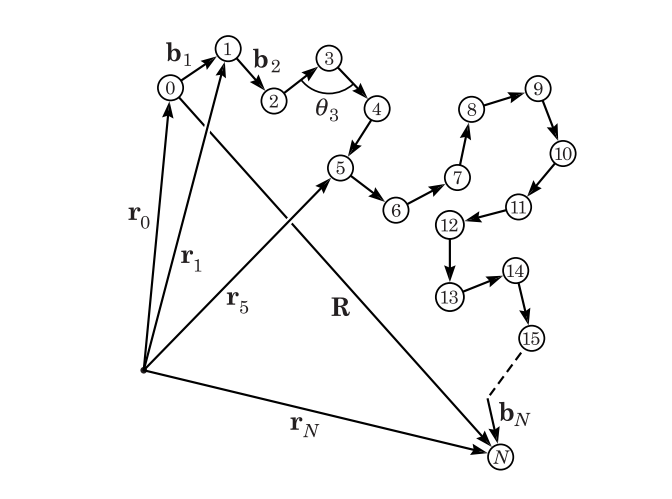
\includegraphics[width=12cm]{./figures/2-1.png}
	\caption{ }
	\label{2.1}
\end{figure}

对于一般含$N+1$个粒子的粗粒聚合物模型,如图(\ref{2.1})所示,单个链的构象配分函数(配分函数是一个平衡态统计物理学中经常应用到的概念,经由计算配分函数可以将微观物理状态与宏观物理量相互联系起来,而配分函数等价于自由能,与路径积分在数学上有巧妙的类似。)可以用类似$Z=\int \exp[-\beta U(\br^{n})] d \br^{N+1}$(1.6)的表示:\\
\begin{equation}
Z_0 = \int \exp[-\beta U_{0}({\br}^{N+1})] ~d \br^{N+1}
\label{2.3}
\end{equation}
其中$\br^{N+1}=(\br_0,\br_1,\ldots,\br_{N})$表示$N+1$粒子的位置,$U_0(\br^{N+1})$是与聚合物特定构型相关联的势能(下标$0$用来表示我们正在讨论单个理想链的性质)。$\int d\br^{N+1}$是三维区域内$N+1$粒子所占体积积分的缩写。对于理想链模型,$U_0$只包含反映短程干扰的相互作用势项。\\

在构象空间中观测点$\br^{N+1}$的联合概率密度是波尔兹曼(Boltzmann)分布(也叫吉布斯分布,是一种覆盖系统各种状态的概率分布、概率测量或者频率分布。当有保守外力(如重力场、电场等)作用时,气体分子的空间位置就不再均匀分布了,不同位置处分子数密度不同。玻尔兹曼分布律是描述理想气体在受保守外力作用、或保守外力场的作用不可忽略时,处于热平衡态下的气体分子按能量的分布规律):\\
\begin{equation}
P_0(\br^{N+1})=Z_{0}^{-1} \exp[[-\beta U_{0}(\br^{N+1})]
\label{2.4}
\end{equation}
此概率权重(或密度)被规范化,以便$\int P_0(\br^{N+1}) d\br^{N+1}=1$。在链的所有配置上,任意函数$f(\br^{N+1})$的系综平均值可以写成\\
\begin{equation}
\langle f(\br^{N+1})\rangle _0 =  \int P_0(\br^{N+1})f(\br^{N+1})~d\br^{N+1}
\label{2.5}
\end{equation}
另一种表示$N+1$粒子链构象自由度的方法是保留一个描述聚合物整体位置的“外部”坐标和$N$个“内部”坐标。一个特别方便的选择是链端的位置,例如,以及图\ref{2.1}所示的$N$ 个键向量,$\bb^{N}=(\bb_1,\bb_2,\ldots,\bb_{N})$,其中$\bb_{i}=\br_{i}-\br_{i-1}$。在聚合物没有外部势作用的情况下,$U_0$只依赖于内部坐标$\bb^{N}$。将$\br^{N+1}$和$(\br_0,\bb^{N})$ 进行雅克比变换,(\ref{2.3}-\ref{2.4})可重新表示为\\


\begin{equation}
Z_0 = V \int \exp[-\beta U_{0}(\bb^{N})]~d\bb^{N}
\label{2.6}
\end{equation}
\begin{equation}
P_0(\br_0,\bb^{N})=Z_{0}^{-1} \exp[[-\beta U_{0}(\bb^{N})]
\label{2.7}
\end{equation}
因此,在链端位置$\br_0$分布是均匀的。\\

自由连接链模型是一种非常简单的理想链模型,其中连接连续粒子的键向量被约束为一个固定的长度,$|\bb_{i}|=b$,但$N$个键向量的方向是各向同性独立分布的。在无限刚性弹簧的极限情况下,$U_0(\bb^{N})$的弹簧模型原则上可以实现固定键长的约束。一个更简单的方法是采用一个$\bb^{N}$表示法,这样约束就会自动得到满足。另
$\bb_{i}=b\bm{n}_{i}$,其中$\bm{n}^{N}=(\bm{n}_1,\bm{n}_2,\ldots,\bm{n}_{N})$是单位球面上一组均匀独立分布的$N$个单位向量。因此,对于自由连接链模型\\

\begin{equation}
P_0(\br_0,\bm{n}^{N})=\frac{1}{V} (\frac{1}{4 \pi})^{N}
\label{2.8}
\end{equation}
它是规范化的,所以$\int d\br_0\int P_0(\br_0,\bm{n}^{N})d\bm{n}^{N}=1$,其中$\int d\bm{n}^{N}$表示单位球面上的$N$个积分。\\
应用上式,我们可以检验自由连接链的各种统计性质。特别是端到端向量$\bbR=\br_{N}-\br_0$的矩,还可以写为$\bbR=\sum _{i=1}^{N} \bb_{i}=b \sum _{i=1}^{N} \bm{n}_{i}$.
$\bm{n}_{i}$的各向同性分布意味着$\langle \bm{n}_{i}\rangle _{0}=0$,因为在每点概率相同,$\bm{n}_{i}$分布在各个方向上,相互抵消,因此$\bbR$的一阶矩消失\\
\begin{equation}
\langle \bbR \rangle_{0}=0
\label{2.9}
\end{equation}
端到端的二阶矩可以写出来\\
\begin{equation}
\langle \bbR_{\alpha} \bbR_{\beta}\rangle_{0}=b^2 \sum _{i=1}^{N} \sum _{j=1}^{N} \langle n_{i \alpha},n_{j \beta} \rangle_{0}
\label{2.10}
\end{equation}
这里我们用希腊下标来表示向量和张量的笛卡尔分量。当$i\neq j$双和项由于各单位向量的独立性而明显消失。对角线项用$\langle n_{i \alpha},n_{j \beta} \rangle_{0}=(1/3)\delta_{\alpha  \beta }$计算,其中$\delta_{\alpha \beta }$是克罗内克(Kronecker)符号,因此:\\
\begin{equation}
\langle \bbR_{\alpha} \bbR_{\beta}\rangle_{0}=\frac{b^{2}N}{3}\delta_{\alpha \beta }
\label{2.11}
\end{equation}
所以自由连接链模型的均方端到端向量完全符合理想链标度定律$R~bN^2,\nu=1/2,N \rightarrow \infty $(2.1):\\
\begin{equation}
R\equiv \sqrt{\langle \bbR \cdot \bbR\rangle _{0}}=bN^{1/2}
\label{2.12}
\end{equation}
注意,上式是在不施加$N\rightarrow \infty$的情况下导出的,(2.1)中省略的标度系数对于自由连接链是完全统一的。\\

端到端向量的更高矩也可以同样计算出来。例如\\
\begin{equation}
\langle (\bbR \cdot \bbR)^2 \rangle_{0}=\frac{5}{3}b^4N(N-\frac{2}{5})
\label{2.13}
\end{equation}
从这个结果可以看出,自由连接链的端到端向量$\bbR$的概率分布不是简单的高斯分布,因为对于这种分布(见附录B)$\langle (\bbR \cdot \bbR)^2 \rangle=\langle (\bbR \cdot \bbR) \rangle^2+2\langle (\bbR \bbR)\rangle:\langle (\bbR \bbR)\rangle$,这导致$\langle (\bbR \cdot \bbR)^2 \rangle_{0}=(5/3)b^4N^2$。但是,对于$N\rightarrow \infty$,上式中给出的四阶矩与高斯分布是一致的。\\

衡量聚合物链平均尺寸的另一个重要指标是回转半径$R_{g}$。这个量是单个片段(粒子)与聚合物质心之间的均方距离,$\bbR_{c}=(N+1)^{-1} \sum _{i=0}^{N} \br_{i}$,即\\
\begin{equation}
R_{g}^2 \equiv \frac{1}{N+1} \sum _{i=0}^{N} \langle (\br_{i}- \bbR_{c})^2 \rangle_{0} 
\label{2.14}
\end{equation}
因此$R_{G}^2$代表了质量分布在聚合物线圈中的二阶矩,而且还可以定义为所有聚合物的结构,例如没有链端的环状聚合物。旋转的平方半径可由另一种形式表示\\
\begin{equation}
R_{g}^2=\frac{1}{(N+1)^2} \sum _{i=0}^{N} \sum _{j>i}^{N} \langle (\br_{i}- \br_{j})^2 \rangle_{0} 
\label{2.15}
\end{equation}
这公式特别容易计算。还可以通过将$\br_{i}-\br_{j}$表示为键向量之和来计算自由连接链的表达式,从而得到$\langle (\br_{i}- \br_{j})^2 \rangle_{0}=b^2 |i-j|$。然后对上式中的二重和进行渐近求和,使$N \rightarrow \infty $。\\
\begin{equation}
R_{g}^{2} = \frac{b^2}{(N+1)^2} \sum _{k=1} ^{N} (N+k-1)k=\frac{b^2 N(N+1)(N+2)}{6(N+1)^2}
\end{equation}
\begin{equation}
R_{g}\approx b(N/6)^{1/2}
\label{2.16}
\end{equation}
因此,自由连接链的回转半径比均方端到端向量$R$小$1/\sqrt{6}$。这证明了在$N$足够大时线性聚合物的任何理想链模型都是成立的。\\
\begin{figure}[H]
	\centering   
	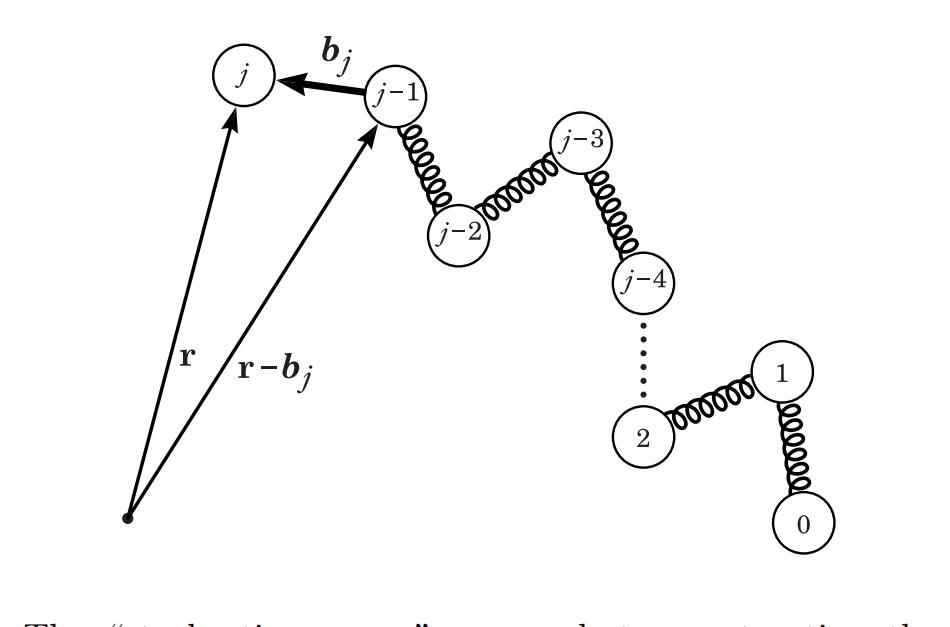
\includegraphics[width=12cm]{./figures/3.png}
	\caption{ }
	\label{2.2}
\end{figure}
图(\ref{2.2})从$j$个粒子链的统计权重出发,用“随机过程”方法建立具有$j+1$粒子的自由连接链末端位置的统计权重。\\

另一种探索理想链模型统计特性的方法不是计算矩,而是直接检测诸如端到端向量等量的概率分布函数。特别是约化分布函数$p_{0}(\br,j)$,它表示含有$j+1$个粒子的聚合物链在其末端$r$位置(粒子标记的$j$)的概率密度。该函数被规范化,以便$\int p_0(\br,j)d\br=1$。在构造这一目标时,我们将有机会在聚合物统计力学与随机过程理论之间建立一个重要的联系。具体来说,连续粒子沿粗粒聚合物链的随机位移类似于离散时间随机过程中在一定时间间隔内发生的随机事件。\\

为了利用随机过程的类比,我们假设一个含有较少粒子的链的末端$p_{0}(\br,j-1)$的概率密度是已知的,如图\ref{2.2}所示,一个$(j+1)$粒子链可以通过添加一个粒子和一个连接键从$j$粒子链中建立。在自由连接链模型中,附加键的长度是固定的,但它的取向与链中已经存在的$j−1$个键的方向无关。因此,我们可以从已知的函数$p_{0}(\br,j)$乘以一个跃迁概率(与所加键的固定长度和均匀方向分布一致)求出概率密度,并对所有可能的键方向进行积分,\\
\begin{equation}
p_{0}(\br,j)=\frac{1}{4 \pi} \int p_0(\br-b \bm{n},j-1)d\bm{n}
\label{2.17}
\end{equation}
这个方程中的因子$1/(4 \pi)$表示与所加键的取向有关的均匀跃迁概率,积分又在单位球面上。这种方程在随机过程理论中称为查普曼-科莫高洛夫(Chapman-Kolmogorov)方程。在这里,自由连接链是一步马尔可夫过程的一个例子,因为跃迁概率只连接链上相邻的粒子。\\

对于解像(\ref{2.17})这样的方程,我们需要一个“初始条件”,指定一个$1$-粒子链的位置分布。然后依次迭代求出$(N+1)$-粒子链末端位置的概率密度$p_{0}(\br,N)$,这种递推格式非常适合于数值计算。就目前的目的而言,(\ref{2.17})可用于推导自由连接链的端到端向量的全部分布函数。\\

为了方便,引入函数$f(\br)$的三维傅里叶变换(与傅里叶分析有关的定义和公式在附录$A$中)\\
\begin{equation}
\hat{f}(\bk)=\int e^{-i\bk \cdot \br}f(\br)~d\br
\label{2.18}
\end{equation}
给出逆变换\\
\begin{equation}
 f(\br)=\frac{1}{(2 \pi)^3} \int e^{i\bk \cdot \br} \hat{f}(\bk)~d\bk
\label{2.19}
\end{equation}
将傅里叶变换应用于(\ref{2.17})的两边,得到以下表达式:\\
\begin{equation}
\begin{aligned}
\hat{p_0}(\bk,j)&=\frac{1}{4 \pi} \int e^{-ib\bk \cdot \bm{n}} \hat{p_0}(\bk,j-1)d\bm{n} \\&=\frac{1}{4 \pi} \int _{R^3}e^{-ib\bk \cdot \bm{n}} \hat{p_0}(\bk,j-1)d\bm{n} \\&=
\frac{1}{4 \pi} \int _{0}^{2 \pi}d \varphi \int _{0}^{\pi} e^{ib|\bk|\bm{n} cos \theta}sin \theta d \theta \hat{p_0}(\bk,j-1) \\&=\frac{1}{2} \int _{-1}^{1}cos b|\bk|dx \hat{p_0}(\bk,j-1) \\&=j_0(b|\bk|)\hat{p_0}(\bk,j-1)
\label{2.20}
\end{aligned}
\end{equation}
其中$j_0(x) \equiv (sinx)/x$是常见的球面贝塞尔函数。依次地将这个方程应用于$j=1,2,\ldots,N$得到\\
\begin{equation}
\hat{p_0}(\bk,N)=[j_0(b|\bk|)]^{N}\hat{p_0}(\bk,0)
\label{2.21}
\end{equation}
特别有趣的情形是对应于初始条件$p_0(\br,0)=\delta(\br)$,其中$\delta(\br)$是三维狄拉克函数(狄拉克函数是由性质定义的广义函数,对于任何函数成立,另见附录$A$)。这意味着链的起始端(粒子$0$) 被约束于原点。有了这种选择,$\hat{p_0}(\bk,0)=1$,$p_0(\bbR,N)$可以解释为含有$N$个键和端到端向量的自由连接链的概率密度。因此\\
\begin{equation}
p_0(\bbR,N)=\frac{1}{(2 \pi)^3 }\int e^{i\bk \cdot \bbR}[j_0(b|\bk|)]^{N}d\bk
\label{2.22}
\end{equation}
是端到端向量的概率密度的精确闭型表达式。当$N\gg1$且$|\bbR| \ll Nb $时,对这个积分的渐近分析证实了我们先前观察到的$\bbR$的二阶和四阶矩与高斯分布是一致的。\\
\begin{equation}
p_0(\bbR,N) \approx [3/(2 \pi Nb)]^{3/2}exp[-3|\bbR|^2/(2Nb^2)]
\label{2.23}
\end{equation}
构象熵的重要概念体现在上式中。在自由连接链的全相空间分布函数$P_0(\br_0,\bb^{N})$与端到端向量的约化概率分布函数$p_0(\bbR,N)$转换的过程中,我们固定端到端向量$\bbR=\sum _{i=1}^{N} \bb_{i}$,在所有固定长度键向量$b$上进行了积分。这种集成相当于对构象状态的枚举。由于在自由连接的模型中,所有的状态都以均匀的概率发生,所以结果是对约束端到端向量$\bbR$的链的自由能的纯粹熵表现:\\
\begin{equation}
F_0(\bbR)=-k_{B}Tlnp_0(\bbR,N)\approx \frac{3k_{B}T}{2Nb^2}|\bbR|^2
\label{2.24}
\end{equation}
这个表达式中的二次项依赖于链的扩张维R可以看作是一个“熵弹簧”势。对于具有较大扩展的链,可用的构象态较少,因此自由能随的增加而增加。此外,$\frac{3k_{B}T}{Nb^2}=\frac{k_{B}T}{2R^2_{g}}$的“弹簧常数”与聚合物线圈尺寸的平方成反比。\\

最后一个主题涉及到自由连接链模型在理想条件下对真实链的适用性。在短尺度(约$1nm$)上,自由连接链明显地简化了真实聚合物链的键合和空间约束,该链仅在一定距离$b$上包含局部键刚性。然而,在较大的尺度上,即$5-10nm$,真实的柔性聚合物在理想状态下表现出符合(\ref{2.12})的自由连接链的标度行为。因此,我们可以通过定义一个等效的自由连接链来描述这类聚合物的介观统计特性。即要求处于理想状态的真实聚合物具有相同的均方端到端向量$R^2=Nb^2$,最大端到端距离$\bbR_{max}=Nb$作为等效的自由连接链。然后,自由连接链的两个参数可以用实验测量或$R^2=\langle \bbR \cdot \bbR\rangle_{0}$和$R_{max}$的估计来表示\\
\begin{equation}
b=R^2/R_{max},N=R_{max}^{2}/R^2
\label{2.25}
\end{equation}
按照这一程序,等价链的键长$b$称为库恩段长度,对大多数乙烯基聚合物而言约为$1nm$。等价链的有效“库恩段”的个数$N$通常比实际链的骨架键数小$50$倍。\\

显然,(\ref{2.25})中给出的将理想状态下的真实链映射到自由连接模型上的条件并不是唯一的。高度扩展的链构象是非常罕见的,因此在实链和等价链之间匹配$R_{max}$的理由是很弱的。定义等效自由连接链的其他方法通常涉及$N$的定义,然后通过匹配实链和等价链之间的$R^2$(或$R_{g}^{2}$)来计算$b$。$N$的一般定义包括每条链的单体重复单位的平均数目,或每条具有规定分子量的链段的平均数目(这可能与实际的化学重复单位相对应,也可能不对应)。从这些过程中获得的$b$值通常称为统计段长度。需要注意的是,$b$和$N$的值将因定义等价链所用的标准而有所不同。然而,所建立的链模型一般都能很好地描述真实聚合物链在理想状态下的介观$(1nm)$统计特性,而不考虑所应用的准则。\\

在本专著中,我们将采用一种比较随意的语言来引用粗粒度、等价链模型中的参数。$n$将可互换地描述为聚合度、每个链的单体数或统计段数。同样,$b$将被称为库恩长度,统计段长度,或单体长度。\\
\endinput

\subsection{珠弹簧(bead-spring)模型}
\begin{center}
\author{hzj}
\end{center}


另一类要的理想链模型是所谓的珠弹簧模型,在这些模型中,沿粗粒链的连续粒子被“弹簧电势(spring potentials)”所束缚,这些弹簧电势有多种形式被选择。定义这些模型的势能$U_{0}$是最合适表达键向量的术语。因此,配分函数和相空间分布函数的$(N+1)$个粒子链(见图\ref{2.1})通常被写成公式(\ref{2.6})-(\ref{2.7})的形式。如果这样一个链的N键全部等价和没有外场的干扰,这些势能可以表示为:
\begin{equation}\label{2.26}
\begin{split}
U_{0}(\bb^{N})= \sum_{i=1}^{N}h(|\bb_{i}|)
\end{split}
\end{equation}
其中$h(x)$是沿高分子聚合物相邻粒子的弹簧电势,因此得出的结论是:
\begin{equation}\label{2.27}
Z_{0}=V(\int \exp[-\beta h(|\mathbf{b}|)]~d\mathbf{b})^N 
\end{equation}
\begin{equation}\label{2.28}
\begin{split}		
P_{0} (r_{0},\mathbf{b}^N) =V^{-1} \prod_{i=1}^{N} \frac{\exp[-\beta h(|\mathbf{b}_{i}|)]}{\int \exp[-\beta h(|\mathbf{b}_{i}|)]~d \mathbf{b}_{i}}
\end{split}
\end{equation}
因此,每个键向量$\mathbf{b}_{i}$都是独立分布的,其统计权重与$\exp[-\beta h(|\mathbf{b}_{i}|)]$成正比。 

它仍然需要指定键h弹簧电势的函数形式。最常见的选择是定义所谓的离散高斯链模型的谐波键电势(harmonic bond potential): 
\begin{equation}\label{2.29}
h(x)=\frac{3k_{B}T}{2b^2} x^2  
\end{equation}
这个电势的参数b,可以被理解为键的均方根长度,因为对任意键i 
\begin{align}\label{2.30}
\begin{split}
<\mathbf{b}_{i}.\mathbf{b}_{i}>_{0}&= \frac{\int_{-\infty}^{\infty} (\mathbf{b}_{i}.\mathbf{b}_{i})~\exp[-\beta h(|\mathbf{b}_{i}|)])~d\mathbf{b}_{i}}{\int_{-\infty}^{\infty} \exp[-\beta h(|\mathbf{b}_{i}|)]~d\mathbf{b}_{i}}\\ &=\frac{\int_{-\infty}^{\infty}\int_{-\infty}^{\infty}\int_{-\infty}^{\infty}(x_1^2+x_2^2+x_3^2)e^{-\frac{3}{2b^2}(x_1^2+x_2^2+x_3^2)}~dx_1dx_2dx_3}{\int_{-\infty}^{\infty}\int_{-\infty}^{\infty}\int_{-\infty}^{\infty}~e^{[-\frac{3}{2b^2}(x_1^2+x_2^2+x_3^2)]}~dx_1dx_2dx_3}\\ &=\frac{3\int_{-\infty}^{\infty}\int_{-\infty}^{\infty}\int_{-\infty}^{\infty}~x_1^2e^{[-\frac{3}{2b^2}(x_1^2+x_2^2+x_3^2)]}~dx_1dx_2dx_3}{\int_{-\infty}^{\infty}\int_{-\infty}^{\infty}\int_{-\infty}^{\infty}~e^{[\frac{-3}{2b^2}(x_1^2+x_2^2+x_3^2)]}~dx_1dx_2dx_3}\\ &=\frac{3 \times\frac{1}{2} (\frac{2b^2}{3})^{3/2}\sqrt{\pi}}{(\frac{2b^2\pi}{3})^{\frac{1}{2}}}\\ &=b^2
\end{split}
\end{align}
其中,所需的高斯积分是附录B中给出的公式的。

离散高斯链的均方端到端向量可以类似的计算,特别的:
\begin{equation}\label{2.31}
<\mathbf{R}\cdot\mathbf{R}>_{0}=\sum_{i=1}^{N}\sum_{i=1}^{N}<\mathbf{b}_{i}\cdot\mathbf{b}_{i}>_{0}
\end{equation}
在这个表示当中,当$i\neq j$时,独立分布的键向量不存在,当$i\neq j$时,$<\mathbf{b}_{i}\cdot\mathbf{b}_{j}>_{0}=<\mathbf{b}_{i}>_{0}<\mathbf{b}_{j}>_{0}=0$。因此
\begin{equation}\label{2.32}
<\mathbf{R}\cdot\mathbf{R}>_{0}=N<\mathbf{b}_{i}\cdot\mathbf{b}_{i}>_{0}=Nb^2
\end{equation}
并精确的恢复了公式((\ref{2.12})的理想链标度,$R=bN^\frac{1}{2}$,除了将b作为自由连接模型固定键长与离散高斯模型的均方根外,我们发现这两个理想模型均方端到端向量的表达是一致的。这容易证明回璇半径$R_{g}$是等价的。因此公式(\ref{2.16})也可以适用离散高斯链。
\begin{figure}[H]
\centering
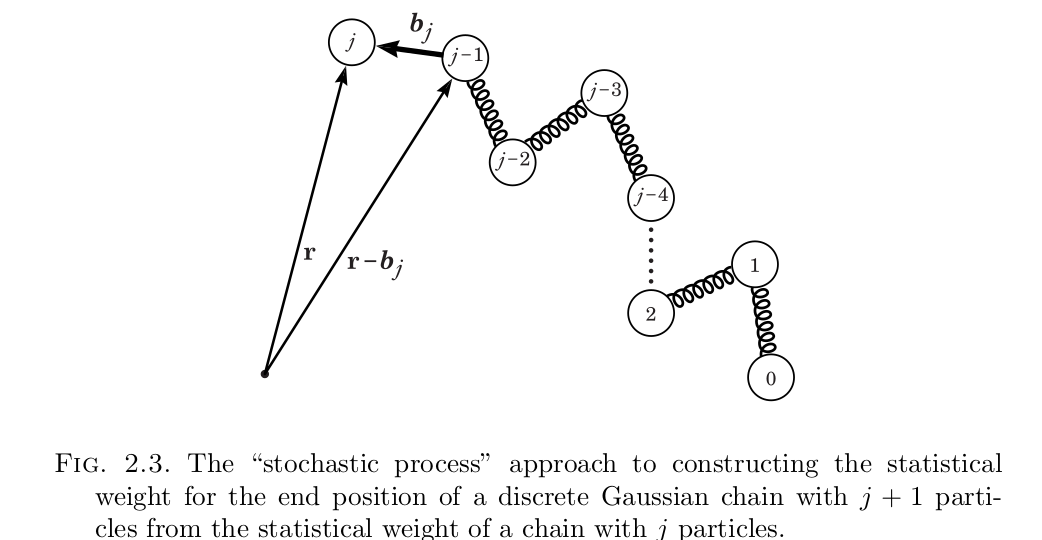
\includegraphics[width=15cm]{./figures/23.png}
\caption{"随机过程”方法构造离散高斯链的末端的统计权重,其中j+1粒子来自j粒子的统计权重。}
\label{figures23}
\end{figure}


为了更充分的探索自由链接和离散高斯链模型的关系,利用随机过程的联系是非常有用的。关于自由连接链,我们考虑约化分布函数$P_{0}(\mathbf{r},j)$,表示在r位置观察(j+1)--粒子链末端粒子j的概率密度。假设一条链的概率密度比它少一个粒子$p_{0}(\mathbf{r},j-1)$,如图\ref{figures23}所示,通过Chapman-Kolmogorov公式建立:
\begin{equation}\label{2.33}
P_{0}(\mathbf{r},j)=\int  \varPhi (\mathbf{b}_{j};\mathbf{r}-\mathbf{b}_{j})~p_{0}(\mathbf{r}-\mathbf{b}_{j},j-1)~d\mathbf{b}_{j}
\end{equation}
在这个表达式中$\varPhi (\mathbf{b}_{j};\mathbf{r}-\mathbf{b}_{j})$是连续粒子j和j-1键向量假设在$\mathbf{b}_{j}$的条件概率密度,给出粒子j-1在$\mathbf{r}-\mathbf{b}_{j}$位置。这是规范化的,因此$\int  \varPhi (\mathbf{b}_{j};\mathbf{r}-b\mathbf{b}_{j})~d\mathbf{b}_{j}=1$。不在任何外场的离散高斯链,$\varPhi$是链上粒子指数j(即随机过程是“平稳的”)和起始位置$\mathbf{r}-\mathbf{b}_{j}$上独立,因此,条件转移概率密度只反映键位移的高斯分布:
\begin{equation}\label{2.34}
\begin{split}
\begin{aligned}
\varPhi(\mathbf{b}_{j};\mathbf{r}-\mathbf{b}_{j})=\varPhi(\mathbf{b}_{j})&=\frac{\exp[-\beta h(|\mathbf{b}_{j}|)]}{\int \exp[-\beta h(|\mathbf{b}_{j}|)]~d\mathbf{b}_{j}} \\ &=(\frac{3}{2 \pi b^2})^{\frac{3}{2}}~\exp[-3|\mathbf{b}_{j}|^2 / (2b^2)]
\end{aligned}
\end{split}
\end{equation}
公式(\ref{2.33})易于用Fourier变换求解,因为离散高斯链$\varPhi$转移概率形式意味着右边是一个三维的卷积积分公式(见附录A)。因此公式(\ref{2.33})的Fourier变换得到Fourier变换的乘积
\begin{equation}\label{2.35}
\hat{p}_{0}(\mathbf{k},j)=\hat{\varPhi}(\mathbf{k})\hat{p}_{0}(\mathbf{k},j-1)
\end{equation}
对$j=1,2,\dots ,N$归纳递推得:
\begin{equation}\label{2.36}
\hat{p}_{0}(\mathbf{k},N)=[\hat{\varPhi}(\mathbf{k})]^N\hat{p}_{0}(\mathbf{k},0)
\end{equation}
公式(\ref{2.34})中的高斯转移概率的Fourier变换是高斯的$^{11}$。$\hat{\varPhi}(\mathbf{k})=\exp(-b^2|\mathbf{k}|^2/6)$,因此公式(\ref{2.36})的离散高斯链可以化简为:
\begin{equation}\label{2.37}
\hat{p}_{0}(\mathbf{k},N)=\exp(-R_{g}^2|\mathbf{k}|^2)\hat{p}_{0}(\mathbf{k},0)
\end{equation}
这里写$R_{g}=\sqrt{Nb^2/6}$作为链的回旋半径来计算,最后,我们专门讨论粒子0约束原点$p_{0}(\mathbf{r},0)=\delta(\mathbf{r})$的情况。其中$\hat{p}_{0}(\mathbf{k},0)=1$,则公式(\ref{2.37})的Fourier逆变换可以写成:
\begin{equation}\label{2.38}
p_{0}(\mathbf{R},N)=[3/(2\pi Nb^2)]^\frac{3}{2}\exp[-3|\mathbf{R}|^2/(2Nb^2)]
\end{equation}

将离散高斯链的这些结果和自由连接链的结果进行比较是很有意思的,特别的,我们发现自由连接链模型公式(\ref{2.21})的精确分布函数$\hat{p}_{0}(k,N)$的Fourier变换与离散高斯链公式(\ref{2.37})不一致,但是对于长度超过b,如:$b|k|<<1$,
\begin{equation}\label{2.39}
[j_{0}(b|\mathbf{k}|)]^N\approx [1-b^2|\mathbf{k}|^2/6+\dots]^N\approx \exp(-R_{g}^2|\mathbf{k}|^2)
\end{equation}
这两个函数是一致符合的。观察的结果是离散高斯链公式(\ref{2.38})是精确的,但是对于自由链接链的结果是近似的(要求$N>>1$且$|\mathbf{R}|<<Nb$)。

离散高斯连模型只是众多可设计的珠弹簧模型之一。这是个特别方便的模型,因为在粗粒键和介观端到端向量的水平上都是高斯的段分布,这便于分析计算各种各样单链的性能。然而,利用连接键的调和势(harmonic potential)的线性(Hookian)弹簧模型有时是不够的。例如:高斯链模型在描述低盐条件下(Netz and Orland,1999)的电解质时,可以表示较大的非物质拉伸。具有延伸特性强的流体力学流动作用下的高斯链也不能代表真实聚合物的无限延伸(Larson,1986)。在这种情况下,可以利用非线性的弹簧模型来防止非物质的扩展链现象。自由连接链也可以被应用,但是由于与固定键长度相关的完整性约束在动态高分子聚合物方案中往往更难实现。(Doi and Edwards,1986).

大部分非均匀聚合物的计算是通过数值计算的观点来实现的,目前使用非线性的珠弹簧模型比较容易,特别是公式(\ref{2.36})适用于所有键相同且其特点是仅取决于键长x的弹簧电势h(x)的任何珠弹簧。$\varPhi(\mathbf{k})$的形式是区分不同链模型的统计特征。一般情况下h(x)的转移概率密度的Fourier变换可以被写为:
\begin{equation}\label{2.40}
\hat{\varPhi(\mathbf{k})}=\frac{\int_{0}^{\infty}  x^2j_{0}(|\mathbf{k}|x)\exp[-\beta h(x)]~dx}{\int_{0}^{\infty}  x^2\exp[-\beta h(x)]~dx} 
\end{equation}
对于公式(\ref{2.29})的线性(高斯)弹簧模型$\hat{\varPhi(k)}=exp(-b^2|k|^2/6)$。比较公式(\ref{2.21})和(\ref{2.36})表明自由连接链模型可以类似的表示:$\hat{\varPhi_{FJ}(k)}=j_{0}(b|k|)$。

作为非线性的珠弹簧模型的例子,考虑类似流变学的计算Warner spring的电势:
\begin{equation}\label{2.41}
h(x)=\frac{2k_{B}T}{2b^2}\frac{x^2}{(1-x^2/b_{0}^2)}
\end{equation}
此电势包含的参数$b_{0}>0$即当$h(x)\to +\infty,x\to b_{0}$键的最大长度,但是,对于弱键的扩张$x/b_{0}<<1$公式(\ref{2.41})减到公式(\ref{2.29})中给定的调和键位电势。因此公式(\ref{2.41})是双参数非线性弹簧定律。它与离散高斯链模型中小键位移的线性定律一致。然而,对于强作用力键长在有限的$b_{0}$处是饱和的。

当被替换公式(\ref{2.40})时,公式(\ref{2.41})的非线性性弹簧模型会导致转换后的转移概率密度$\varPhi_{NL}(k)$可以表示为(wavevector)波矢量和无尺度$b/b_{0}$比的函数,对于$b/b_{0}<0.1$,$\varPhi_{NL}(b|k|,b/b_{0})$与线性弹簧函数$\varPhi_{G}(k)$几乎没差别。 然而,当$b/b_{0}$的值比较大时,非线性弹簧在波矢量中的影响依赖于$\varPhi_{NL}(k)$。图\ref{figures24}比较了离散高斯链、自由连接链和公式(\ref{2.41})的非线性珠弹簧链在$b/b_{0}=1$情况下的转移概率的Fourier变换。非线性弹簧定律对$|k|$具有振幅依赖性,其性质上类似于自由连接链。然而,自由链接模型振幅受到更强的阻尼,其键的长度被严格地约束为b。
\begin{figure}[H]
\centering
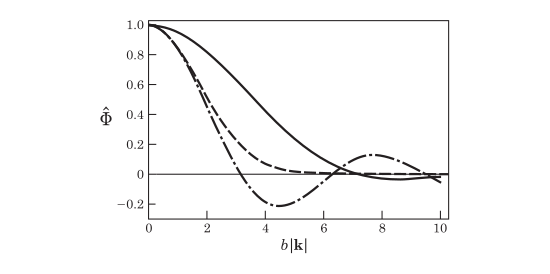
\includegraphics[width=15cm]{./figures/24.png}
\caption{分别是离散高斯(虚线),自由连接链(点虚线)和非线性弹簧模型(实线)的键转移概率$\varPhi_{G}$、$\varPhi_{Fj}$和$\varPhi_{NL}$的Fourier变换,用$b/b_{0}=1$来计算非线性弹簧模型}
\label{figures24}
\end{figure}

\subsection{连续高斯链模型}
连续高斯链是一种用于分析和数值计算的理想链模型,该模型可以被视为离散高斯链模型的连续极限,其中的聚合物被视为一个连续的线性弹性丝(linearly elastic filament)。如图2.5所示,连续高斯链的构型由空间曲线$\mathbf{r}(s)$描述,表示高分子长链上某一链节的位置,其中$s\in [0,N]$,被定义为路径(contour)变量。第$s$个链节在空间中的位置记为$\mathbf{r}(s)$,末端距矢量(end-to-end-vector)$R$可以表达为$R=\mathbf{r}(N)−\mathbf{r}(0)$。
\begin{figure}[H]
\centering
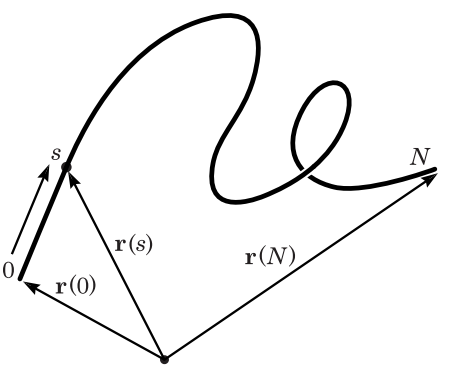
\includegraphics[scale=0.7]{./figures/41.png}
\caption{}
\end{figure}
图2.5:空间曲线$\mathbf{r}(s)$描述连续高斯链模型将聚合物的构型,其中$s\in [0,N]$是路径参数。$\mathbf{r}(0)$和$\mathbf{r}(N)$是链端位置。

连续高斯链的势能可以写成
\begin{gather}
U_0[\mathbf{r}]=\frac{3k_BT}{2b^2}\int_{0}^{N} \mathrm{d}x\left| \frac{d\mathbf{r}(s)}{ds} \right|^2
\end{gather}
其中$b$为链节的统计长度,$U_0[\mathbf{r}]$的方括号符号表示$U_0$是定义聚合物构型的空间曲线$\mathbf{r}(s)$的泛函。泛函是连续函数到数之间的映射。势能的形式与离散高斯链的方程$U_0(\mathbf b^N)=\sum_{i=1}^{N}h(\left|\mathbf{b}_i\right|^2 )$和$h(x)=\frac{3k_BT}{2b^2}x^2$密切相关。如果我们将$\frac{d\mathbf{r}(s)}{ds}$看作高分子长链上第$s$节(链节长度为$ds$)的拉伸形变,则方程$(2.42)$对链的整个路径上每一个这样的微分段的谐波势贡献(harmonic potential contribution)求和。值得注意的是,在连续高斯链模型中,$s$并不表示弧长,而只是表示链上各段的参数指标。因此,拉伸$\frac{d\mathbf{r}(s)}{ds}$不是固定单位向量,它的大小是可以自由波动。势能方程$(2.42)$通常称为“Edwards Hamiltonian”。

连续高斯链的构型配分函数可以写成
\begin{gather}
Z_0=\int \mathcal{D}\mathbf{r}~\exp(-\beta U_0[\mathbf{r}])
\end{gather}
其中$\int \mathcal{D}\mathbf{r}$表示所有可能的描述聚合物的构型的空间曲线$\mathbf{r}(s)$上的泛函积分。这类泛函积分,又称路径积分,是量子力学和概率论领域(Feynman和Hibbs,1965)所熟悉的,其中$\mathbf{r}(s)$对应于量子粒子或布朗(Brownian)粒子在时间$s$的位置。实际上,方程$(2.43)$是经典扩散(brownian motion)路径积分描述中的维纳运动(Wiener motion)。

路径积分是一种复杂的数学对象,在定义和操作上需要一定的精确性(Simon,1979)。然而在这里,我们将非正式地和以物理的方式来研究这些对象。定义路径积分有两种方法,其中一种方法是用$N_s+1$个等距路径点去离散路径,因此我们用$N_s+1$个点的空间位置逼近连续函数$\mathbf{r}(s)$,其中这$N_s+1$个点由向量$(\mathbf{r}_0,\mathbf{r}_1,...,\mathbf{r}_{N_s})$表示。这样,路径积分可以定义为$3(N_s+1)$维的普通积分(假设聚合物在体积为$V$的三维空间中)
\begin{gather}
\int \mathcal{D}\mathbf{r}\approx \prod_{i=0}^{N_s} \int \, \mathrm{d} \mathbf{r}_i
\end{gather}
其中,近似的质量随着$N_s$的增加而提高。当$N_s$有限时,连续高斯链的路径积分近似于有$N_s+1$个珠子的离散高斯链的配分函数。特别是,我们有一个近似
\begin{gather}
Z_0\approx \prod_{j=0}^{N_s} \int \, \mathrm{d} \mathbf{r}_j~\exp \left( -\frac{3}{2b^2\bigtriangleup s}\sum_{i=1}^{N_s}\left|\mathbf{r}_{i-1}-\mathbf{r}_i \right|^2 \right)
\end{gather}
其中,其中一个$N_s$键的均方长度(mean-squared)由$b^2\bigtriangleup s$给出,$\bigtriangleup s=N/N_s$是路径点之间的间距。

方程$(2.45)$的巧妙之处源于连续极限,因为$Z_0$尺度为$VN_s^{−(3/2)N_s}$,当$N_s\rightarrow \infty$时为零。通常我们对平均值感兴趣,它可以表示成两路径积分的比率。例如,连续高斯链的末端距矢量的均方值可以表示为
\begin{gather}
R^2\equiv \left \langle \mathbf{R}\cdot \mathbf{R}\right \rangle _0=\frac{\int \mathcal{D}\mathbf{r}\left| \mathbf{r}(N)-\mathbf{r}(0) \right|^2~\exp(-\beta U_0[\mathbf{r}])}{\int \mathcal{D}\mathbf{r}~\exp(-\beta U_0[\mathbf{r}])}
\end{gather}
其中分母只是配分函数$Z_0$。当根据方程$(2.45)$对上述方程的分子和分母中的路径积分进行离散时,
发现奇异因子完全抵消,从而当$N_s\rightarrow \infty$时,$R^2$更好定义。此外,在路径积分的数值计算中,通常采用有限的$N_s$来避免奇异性。

定义路径积分的另一种方法是通过路径的谱表示(spectral represention)。特别是,我们可以用扩充的一组完整的基函数$\lbrace \phi _0(s),\phi _1(s),... \rbrace$来表示空间曲线$\mathbf{r}(s)$
\begin{gather}
\mathbf{r}(s)=\sum_{p=0}^{\infty} \mathbf{a}_p \phi _p(s)
\end{gather}
这是一种广义的傅里叶展开式,其展开式系数$\mathbf{a}_p$可以看作是广义傅里叶系数(见附录A)。对于在流体介质中自由悬浮(freely suspended in a fluid medium)的聚合物,基函数的一种方便的选择是符合“无拉伸”(no-stretch)边界条件的余弦集$\frac{d\mathbf{r}(s)}{ds}\vert _{s=0}=\frac{d\mathbf{r}(s)}{ds}\vert _{s=N}=0$。这相当于余弦傅里叶级数表示
\begin{gather}
\mathbf{r}(s)=\mathbf{a}_0+2\sum_{p=1}^{\infty} \mathbf{a}_p \cos(p\pi s/N)
\end{gather}
根据这些基函数的正交性可以求解傅里叶系数
\begin{gather}
\mathbf{a}_p=\frac{1}{N}\int_{0}^{N}  \mathrm{d}s~\cos(p\pi s/N)\mathbf{r}(s),p=0,1,2,...,\infty
\end{gather}
这些模型在聚合物文献中被称为Rouse模型,在聚合物动力学理论中起着特别重要的作用(Doi和Edwards,1986)。实际上,$\mathbf{a}_0$可以解释为聚合物质心的位置,而$\mathbf{a}_p,p=1,2,3,...$,尺度越细则提供更多关于聚合物形状的信息。

利用Rouse谱表示,聚合物的所有构型(路径)上的积分可以解释为对所有Rouse模型的积分的乘积。
\begin{gather}
\int \mathcal{D}\mathbf{r}= \prod_{p=0}^{\infty} \int \, \mathrm{d} \mathbf{a}_p
\end{gather}
上述表达式右手边的对象是一个无穷维积分,所以我们再次遇到了配分函数$Z_0$的存在性问题。然而,这两个路径积分的比率证明是有限的,
为了数值计算的目的,我们取有限$P\gg1$使路径积分正则化(消除奇异点)
\begin{gather}
\int \mathcal{D}\mathbf{r}\approx \prod_{p=0}^{P} \int \, \mathrm{d} \mathbf{a}_p\end{gather}
为了说明Rouse模型在连续高斯链计算中的应用,用Rouse模型表示末端距矢量的均方值是
\begin{gather}
\left | \mathbf{r}(N)-\mathbf{r}(0) \right |^2=16\sum_{p=1,3,...}^{\infty}\sum_{q=1,3,...}^{\infty} \mathbf{a}_p \cdot \mathbf{a}_q
\end{gather}
这个数的均值可以写为
\begin{gather}
\left \langle \left| \mathbf{R} \right|^2 \right \rangle _0=16\sum_{p=1,3,...}^{\infty}\sum_{q=1,3,...}^{\infty} \left \langle \mathbf{a}_p \cdot \mathbf{a}_q \right \rangle _0
\end{gather}
其中,在Rouse模型中定义对象$f(\mathbf{a})$的平均值为
\begin{gather}
\left \langle f(\mathbf{a}) \right \rangle _0=\frac{\begin{matrix} \prod_{p=1}^{\infty} \int \, \mathrm{d} \mathbf{a}_p f(\mathbf{a})\exp(-\beta U_0(\mathbf{a})) \end{matrix}}{\begin{matrix} \prod_{p=1}^{\infty} \int \, \mathrm{d} \mathbf{a}_p \exp(-\beta U_0(\mathbf{a})) \end{matrix}}
\end{gather}
在Rouse模型表达式中,方程$(2.42)$的势能是对角的
\begin{gather}
\beta U_0(\mathbf{a})=\frac{1}{2}\sum_{p=1}^{\infty}\alpha (p)\mathbf{a}_p \cdot \mathbf{a}_p
\end{gather}
其中$\alpha (p)=6\pi ^2p^2/(b^2N)$。注意,质心$p=0$模型是均匀分布。$p>0$模型都是统计独立的,是高斯分布,因此如下有(附录B)
\begin{gather}
\left \langle \mathbf{a}_p \cdot \mathbf{a}_q \right \rangle _0=\frac{3}{\alpha (p)}\delta _{pq}
\end{gather}
替换到方程$(2.53)$将得
\begin{gather}
\left \langle \left| \mathbf{R} \right|^2 \right \rangle _0=\frac{8b^2N}{\pi ^2}\sum_{p=1,3,...}^{\infty}\frac{1}{p^2}=b^2N
\end{gather}
由此我们得出结论:连续高斯链具有离散高斯链的性质,它的末端距矢量的均方值由$R=bN^{1/2}$给出。类似用期望公式给出连续高斯链的卷积公式$R_g=b(N/6)^{1/2}$。

\begin{figure}[H]
\centering
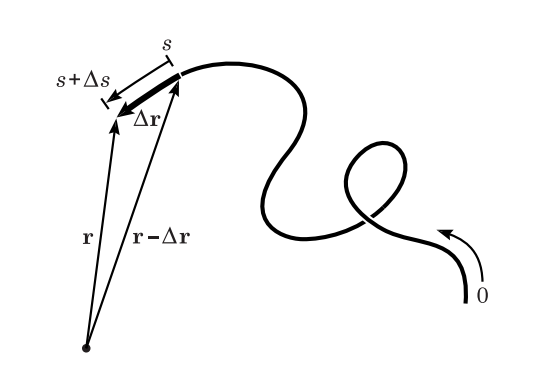
\includegraphics[scale=0.7]{./figures/42.png}
\caption{}
\end{figure}

图2.6;用“随机过程”(stochastic process)方法从具有$s$段的连续高斯链的统计权重中构造出具有$s+\bigtriangleup s$段的连续高斯链末端位置的统计权重。

在探索连续高斯链模型的性质时,我们现在回到了随机过程方法。具体来说,考虑一个约化的分布函数$p_0 (\mathbf{r},s)$是很有用的,它描述了在$\mathbf {r}$处,一个连续的路径长度为$s$的高斯链。这个函数满足归一化条件的,即$\int \, \mathrm{d} \mathbf{r}~p_0(\mathbf{r},s)=1$。通过对离散高斯链的方程$p_0(\mathbf{r},j)=\int \, \mathrm{d} \mathbf{b}_j~\Phi(\mathbf{b}_j;\mathbf{r}-\mathbf{b}_j)p_0(\mathbf{r}-\mathbf{b}_j,j-1)$的类比,我们可以通过Chapman-Kolmogorov方程利用非常小的链的信息建立分布函数
\begin{gather}
p_0(\mathbf{r},s+\bigtriangleup s)=\int \, \mathrm{d}(\bigtriangleup \mathbf{r})\Phi(\bigtriangleup \mathbf{r};\mathbf{r}-\bigtriangleup \mathbf{r})p_0(\mathbf{r}-\bigtriangleup \mathbf{r},s)
\end{gather}

图2.6说明了上述方程的物理内容,它依赖于连续链的最后一部分离散化。转移概率密度$\Phi(\bigtriangleup \mathbf{r};\mathbf{r}-\bigtriangleup \mathbf{r})$描述了路径长度$\bigtriangleup s$的链段的位移为$\bigtriangleup \mathbf{r}$的条件概率,从路径位置$s$处的$\mathbf{r}-\bigtriangleup \mathbf{r}$开始。连续高斯链的相关随机过程是稳定的,所以$\Phi =\Phi(\bigtriangleup \mathbf{r})$与起始位置和路径位置无关。$\Phi(\bigtriangleup \mathbf{r})$的表达式直接来自于连续高斯链方程$(2.45)$之前的离散化:
\begin{gather}
\Phi(\bigtriangleup \mathbf{r})=\left( \frac{3}{2\pi b^2 \bigtriangleup s} \right)^{3/2}\exp \left(- \frac{3\left| \bigtriangleup \mathbf{r} \right|^2}{2b^2 \bigtriangleup s} \right)
\end{gather}
连续链模型的一个有用的特点是,Chapman-Kolmogorov积分方程可以归结为偏微分方程,在概率论中可归结为Fokker-Planck方程(van Kampenn,1981)和量子理论中的Feynman-Kac公式(Feynman和Hibbs,1965)。我们通过导出与方程$(2.58)$相结合的Fokker-Planck方程来说明这一点。这一推导是方程的两边通过泰勒展开。注意到在这种情况下,$\Phi(\bigtriangleup \mathbf{r};\mathbf{r}-\bigtriangleup \mathbf{r})$与初始位置$\mathbf{r}-\bigtriangleup \mathbf{r}$无关,我们不扩展转移概率。有
\begin{equation}
\begin{aligned}
p_0(\mathbf{r},s)+\bigtriangleup s\frac{\partial}{\partial s}p_0(\mathbf{r},s)+O(\bigtriangleup s^2)=&p_0(\mathbf{r},s)-\left \langle \bigtriangleup \mathbf{r} \right \rangle _\Phi \cdot \bigtriangledown p_0 (\mathbf{r},s)\\ &+\frac{1}{2!}\left \langle \bigtriangleup \mathbf{r}  \bigtriangleup \mathbf{r} \right \rangle _\Phi:\bigtriangledown \bigtriangledown p_0(\mathbf{r},s)\\ &+O(\left \langle \bigtriangleup \mathbf{r}  \bigtriangleup \mathbf{r}  \bigtriangleup \mathbf{r} \right \rangle _\Phi)
\end{aligned}
\end{equation}
其中,该方程中出现的$\Phi$平均定义为
\begin{gather}
\left \langle f(\bigtriangleup \mathbf{r}) \right \rangle _\Phi = \int \, \mathrm{d}(\bigtriangleup \mathbf{r})\Phi (\bigtriangleup \mathbf{r})f(\bigtriangleup \mathbf{r})
\end{gather}
利用方程$(2.59)$的显式高斯形式,可以将方程$(2.60)$右侧的平均值计算为(附录B)
\begin{gather}
\left \langle \bigtriangleup \mathbf{r} \right \rangle _\Phi = 0
\end{gather}
\begin{gather}
\left \langle \bigtriangleup \mathbf{r}_\alpha \bigtriangleup \mathbf{r}_\beta \right \rangle _\Phi = \frac{b^2 \bigtriangleup s}{3}\delta_{\alpha \beta}
\end{gather}
如果我们将这些式子带入方程$(2.60)$中,则$\bigtriangleup s \rightarrow \infty$时的分布函数$p_0(\mathbf{r},s)$满足Fokker-Planck方程

\begin{gather}
\frac{\partial}{\partial s}p_0(\mathbf{r},s)=\frac{b^2}{6}\bigtriangledown ^2 p_0(\mathbf{r},s)
\end{gather}

因此,连续高斯链的Fokker-Planck方程给出的具有“扩散系数”$b^2/6$
的传统扩散方程的形式。该方程的解提供了关于端点段$p_0(\mathbf{r},s)$分布的完整信息。

Fokker-Planck方程是特别方便,因为有各种各样的分析和数值技术可用于求解偏微分方程。对于方程$(2.64)$,对应于初始条件$p_0(\mathbf{r},s)=\delta(\mathbf{r})$的基本(格林函数)解是
\begin{gather}
p_0(\mathbf{r},s)=\left[ 3/(2 \pi sb^2) \right]^{3/2}\exp \left[ -3\left| \mathbf{r} \right|^2/(2sb^2) \right]
\end{gather}
如果令$s=N,\mathbf{r}=\mathbf{R}$,则末端距矢量恢复成熟悉的高斯分布函数$(2.38)$
在比单键更大的尺度下,离散高斯链和连续高斯链明显具有相同的链端分布函数。使用连续链的优点是它允许用偏微分方程进行计算。这一优势将在第三章中变得更加明显,在第三章中,我们将考虑有外势的链。
\endinput
\subsection{2.5}


\cite{tam19912d}
\bibliography{../ref}
\end{document}
